\documentclass[12pt]{article}
\usepackage[a4paper, margin=1in]{geometry}
\usepackage[utf8]{inputenc}
\usepackage{titlesec}
\usepackage{enumitem}
\usepackage{graphicx}
\usepackage{titling}
\usepackage{longtable}
\usepackage{booktabs}
\usepackage[hidelinks]{hyperref}
\usepackage{fancyhdr}
\usepackage{setspace}
\usepackage{caption}
\usepackage{cite}
\usepackage{amsmath}
\pagestyle{fancy}
\fancyhf{}
\rhead{CSE 816: DevOps}
\lhead{Final Project}
\rfoot{\thepage}
\titleformat{\section}{\normalfont\Large\bfseries}{\thesection}{1em}{}
\titleformat{\subsection}{\normalfont\large\bfseries}{\thesubsection}{1em}{}
\setstretch{1.2}
\pretitle{%
  \begin{center}
    
\includegraphics[width=0.25\textwidth]{logo.jpeg}\\[1em]  % Logo
    \large CSE 816 : Software Production Engineering\\
    \large Final Project \\[2em]  % Some spacing before the main title
    \LARGE
}
\title{\textbf{CSE 816 : SPE Final Project Report}}
\posttitle{\end{center}}
\author{
    AMEDEKA Tsevi Christian: MS2024502
    \\[2\baselineskip]
    \textbf{Instructor: Prof B. Thangaraju}
}
\date{May 2025}

\begin{document}
\maketitle
\newpage
\tableofcontents
\listoffigures
\newpage

\section{Project Description}
This section provides an overview of the project's purpose, goals, and scope. It outlines the motivation behind the project and the specific DevOps practices implemented to achieve the desired outcomes.

\section{System Components}
This section describes each component of the system, including:
\begin{itemize}
    \item Source code repository and version control system: Git and GitHub
    \item CI/CD pipeline tools: Jenkins and GitHub Hooks
    \item Containerization : Docker
    \item Configuration management : Ansible
    \item Monitoring and logging : Grafana and Prometheus
    \item Deployment platform : Kubernetes
\end{itemize}

\section{System Diagram}
This section presents the architecture of the system, showing the interaction between components in the DevOps pipeline.\\
 
\begin{center}
    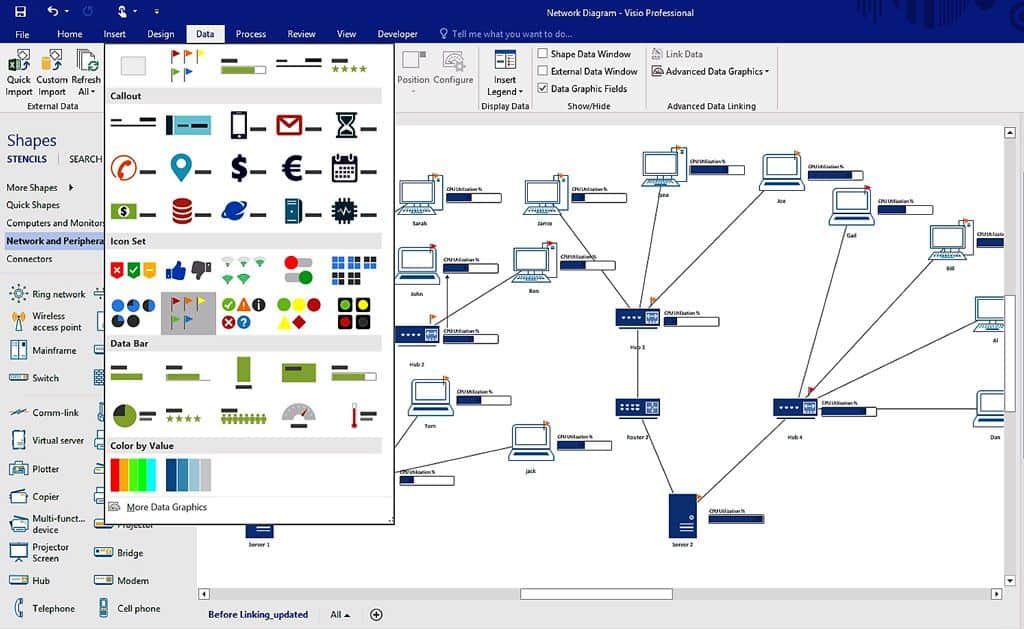
\includegraphics[width=0.9\textwidth]{diagram.png}
    \captionof{figure}{System Architecture Diagram} \label{diagram.png}
\end{center}

\section{Implementation}
This section details the steps taken to implement the system. It includes:
\begin{itemize}
    \item Setting up the repository and initial project structure
    \item Creating and automating the CI/CD pipeline
    \item Building and pushing Docker images
    \item Configuring infrastructure with Ansible
    \item Deploying the application on the target environment
    \item Integrating monitoring tools
\end{itemize}
\bibliographystyle{plain}
\bibliography{Report}

\end{document}